Una volta concluso lo sviluppo del GRIDS System con Blockchain integrata, è indispensabile valutarne le performance.

La metrica che è stata adoperata per la misura delle prestazioni della piattaforma è il ritardo, nello specifico, sono stati misurati tre tipi di delay:

\begin{itemize}
    \item \textit{End-to-end delay}: il tempo che intercorre tra il momento in cui il client effettua la richiesta di dati e quello in cui la transazione viene confermata e l'utente può visualizzare i dati;
    \item \textit{Client-side delay}: il lasso di tempo tra l'invio della richiesta da parte del Client e la ricezione della risposta da parte del Server con l'indirizzo al quale saranno disponibili i dati una volta confermata la transazione;
    \item \textit{Instant buy delay}: l'intervallo di tempo necessario per la ricezione dei dati a partire dalla richiesta di dati con credito residuo.
\end{itemize}

Una considerazione molto importante da fare è che, nel caso delle transazioni "lente", vi è una sorta di problema di "campionamento": visto che nella Testnet i blocchi vengono estratti ogni circa 20 minuti (che scende a 10 nel caso della rete Bitcoin ufficiale), il tempo di ritardo varierà in base a quanto tempo prima è stato risolto l'ultimo blocco della blockchain.

La prima prova è stata effettuata con 100 transazioni  
Ho provato con 100 transazioni standard e alcune di esse sono state respinte per "error 64: too-long-mempool-chain": non entravano più nel mempool perché ha una misura limitata! Vedere https://www.mycryptopedia.com/mempool-ex plained/ per la spiegazione.

The Mempool consists of pending transactions that have occurred over a cryptocurrency’s network and are therefore awaiting approval by a cryptocurrency miner. Each node on a cryptocurrency network operates their own Mempool, and thus will have their own unique size. The size of a node’s Mempool is typically represented as the unit of memory, megabyte (MB).
As there are often thousands of transactions being held in the Mempool, it becomes unclear exactly which transaction miners should select to be included in the next block. Even though the goal is to have all transactions include on the blockchain, one method of getting your transaction included quicker, is to pay a higher fee. By paying a high fee on a transaction, the miner becomes incentivized to include your transaction in the next block rather than a transaction with a much lower fee. This is because miners receive fee payments on each transaction that they add to the blockchain, and therefore, miners will want to maximize the amount of money that they earn. 
The Mempool is prone to fluctuations in size depending how many pending transactions are awaiting confirmation by a miner. Transaction backlog is known to be a frequent issue for a cryptocurrency experiencing large transactions volume across its network. Backlogs tend to occur because there is a limit on the number of transaction that can be included in a block, however, there is no limit on the number of transactions that can occur at any given time. The Mempool essentially becomes the bottle neck of network and it becomes very important that it is properly managed.

In Bitcoin Core\footnote{https://bitcoin.org/en/bitcoin-core/} il limite di transazioni non confermate che si possono generare di seguito è 25, quindi pazienza. Con bitcoinj non è stato implementato ancora un modo per aggirare questo limite, avrebbe addirittura poco senso, dato che il fatto che i nodi siano in modalità SPV va in antitesi con il fatto di poter generare un numero molto grande di transazioni.

Però in ogni caso la piattaforma ha il meccanismo recharge, quindi il problema non si pone...

Un'altra importante precisazione da fare è che il mempool error si può verificare quando è un singolo wallet a generare troppe transazioni di seguito, non quando sono tanti wallet a generare meno transazioni: ciò significa che la rete SIoT non costituisce \textit{bottleneck}. In condizioni di utilizzo normale da parte di un utente qualsiasi, difficilmente saranno mandate così tante richieste...
%%

Provare con 25 trx "lente"

Poi con 100 trx "veloci" (fatto)

E poi vediamo i tre grafici: ritardo client-side delle trx standard, ritardo totale delle trx standard, ritardo totale delle transazioni veloci.

Sui grafici: 

il client side delay tende ad avere una distribuzione normale (il grafico, infatti, ricorda molto la \textit{normal function}). 

le instant buy presentano ritardi molto contenuti, com'era auspicabile. Da notare il punto con ritardo più alto che corrisponde alla prima richiesta.

l'end-to-end delay, infine, presenta valori temporali molto più ampi, visto che è compreso il tempo della conferma delle transazioni. La discontinuità che si osserva nel grafico è causata dal fatto che una parte delle transazioni sono state incluse in un blocco, mentre un'altra parte è stata confermata nel blocco successivo. Quel gradino poi è di 5 minuti perchè ogni tanto nella testnet vengono creati i blocchi a 5 minuti di distanza anche se la media è di 20, è una cosa che succede raramente ma GUARDA CASO L'HO BECCATA durante il testing.

\begin{figure}[h!t]
\centerline{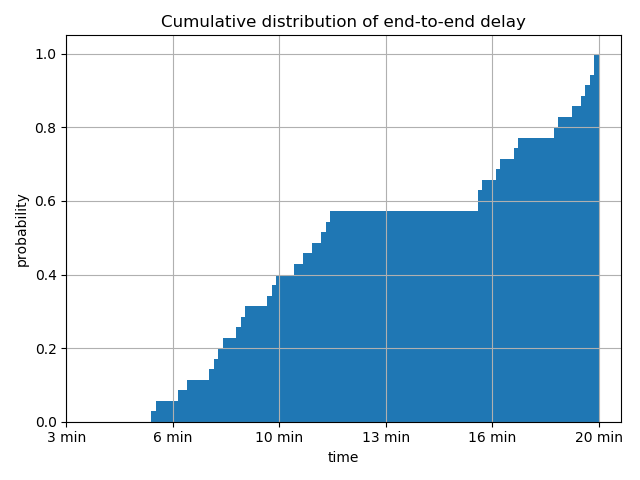
\includegraphics[width=\textwidth]{img/end-to-endGIUSTO}}
\caption{CDF dei delay end-to-end delle transazioni}
\label{f:calcoli:end2end}
\end{figure}

\begin{figure}[h!t]
\centerline{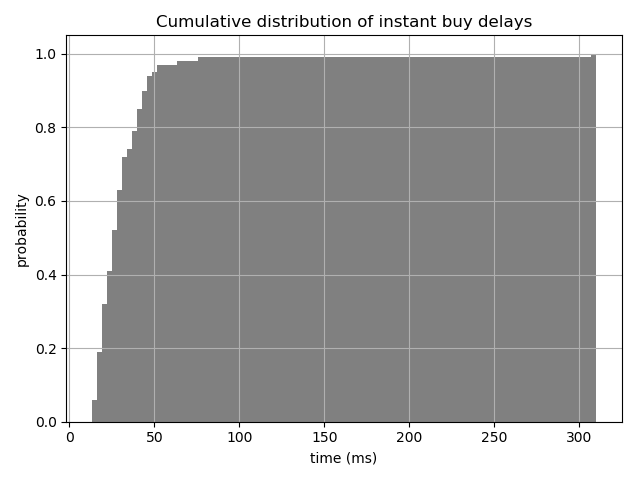
\includegraphics[width=\textwidth]{img/instant-buy-delay-grey}}
\caption{CDF dei delay delle transazioni effettuate con credito}
\label{f:calcoli:instant}
\end{figure}

\begin{figure}[h!t]
\centerline{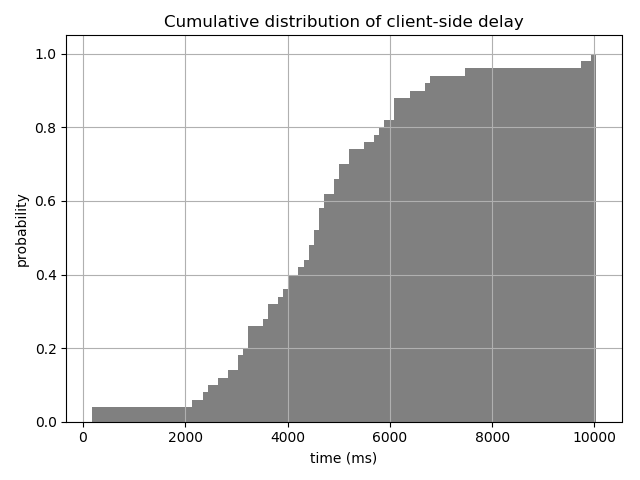
\includegraphics[width=\textwidth]{img/client-side-delay-grey}}
\caption{CDF dei delay client-side delle transazioni}
\label{f:calcoli:client}
\end{figure}